% !TEX root = ../masterthesis.tex
\chapter{Gallium Arsenide Quantum Dots}
\label{chapter:quantum-dot}

\section{General properties and manufacturing}

\begin{figure}[H]
	\centering
	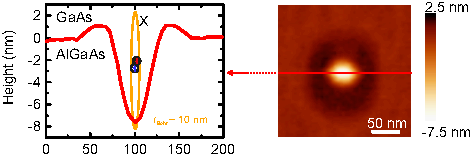
\includegraphics[width=0.9\linewidth]{figures/quantum-dot/QD_plot_AFM}
	\caption{Height profile (red) of a droplet-etched nanohole in an AlGaAs layer is shown in the left image.
	The orange line represents the wavefunction of the exciton which resembles the ground state of an hydrogen atom.
	Because of that the bohr radius $r_{\textrm{Bohr}}$ is denoted.
	The right image shows the atomic force microscopy picture of the nanohole.
	An GaAs quantum dot is obtained after filling the hole with GaAs and avergrowth with AlGaAs~\cite{reindl_highly_2019}}
	\label{fig:qdplotafm}
\end{figure}

\section{Adiabatic rapid passage}

\section{Fine structure splitting}


\section{Exciton emission spectrum}

The discussion of the emission of GaAs quantum dots in the following chapters will be limited to excitonic emission. 
This section will provide the basis for chapter~\ref{chapter:scanning-fabry-perot}.

\subsection{Zero-phonon line and phonon sideband}
The excitonic emission of GaAs quantum dots exhibit non-Lorentzian asymmetric broadening. As shown by \textcite{peter_phonon_2004} this side bands can be traced back to a coupling to acoustic phonons.
The discussion of the phonon sidebands is based on \textcite{friedrich_photochemical_1984} and \textcite{peter_phonon_2004}.

Figure~\ref{fig:line-shape} displays a schematic representation of the zero-phonon line and phonon side band absorption spectrum.
The intensity distribution between the two components depends is strongly dependent on temperature.
\begin{figure}[H]
	\centering
	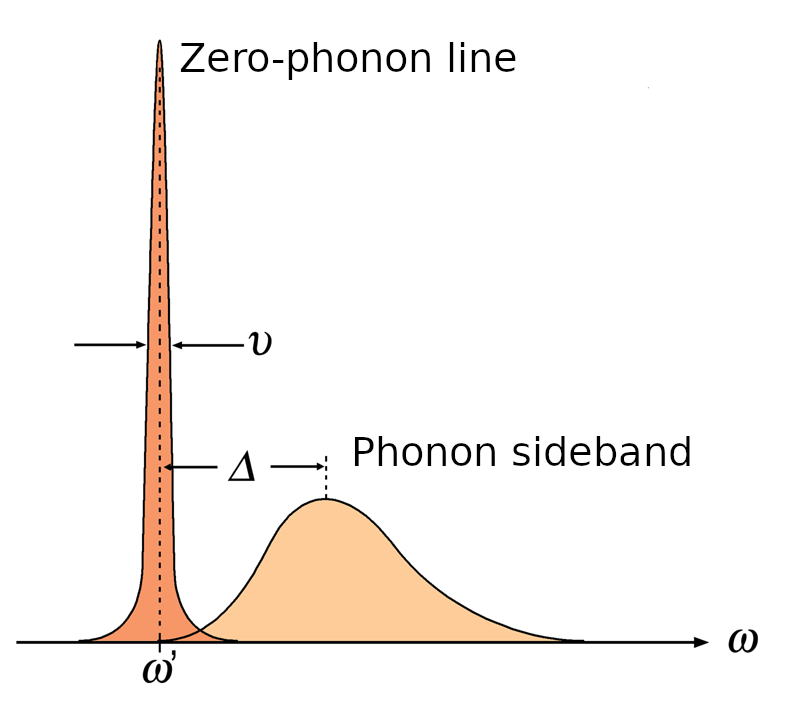
\includegraphics[width=0.6\linewidth]{figures/quantum-dot/Line-shape}
	\caption[Absorption line shape of an electronic excitation.]{Absorption line shape of an electronic excitation.
	The emission is mirrored at $\omega'$.}
	\label{fig:line-shape}
\end{figure}
To determine the frequency gap $\Delta$ the Franc-Condon principles are used. It states that electronic transition between ground and excited state is much faster than the motion in the lattice.
Hence, there is no motion along the configurational coordinates $q_i$ during the energy transitions as depicted in figure~\ref{fig:phonon-energy-diagram}.
The transitions can be displayed as vertical arrows with the shorter arrow describing the zero-phonon line and the longer one describing the phonon sideband.
According to the Franc-Condon principles, the more the wave functions of two vibrational energy levels overlap, the likelier is the electronic transition between these two.
In the case of figure~\ref{fig:phonon-energy-diagram} this occurs when the photon energy equals to the energy difference $E_1-E_0$ plus three quanta of vibrational energy $\hbar \Omega_i$.
The emission follows the same principle.


\begin{figure}[H]
	\centering
	\begin{subfigure}[b]{0.48\textwidth}
		\centering
		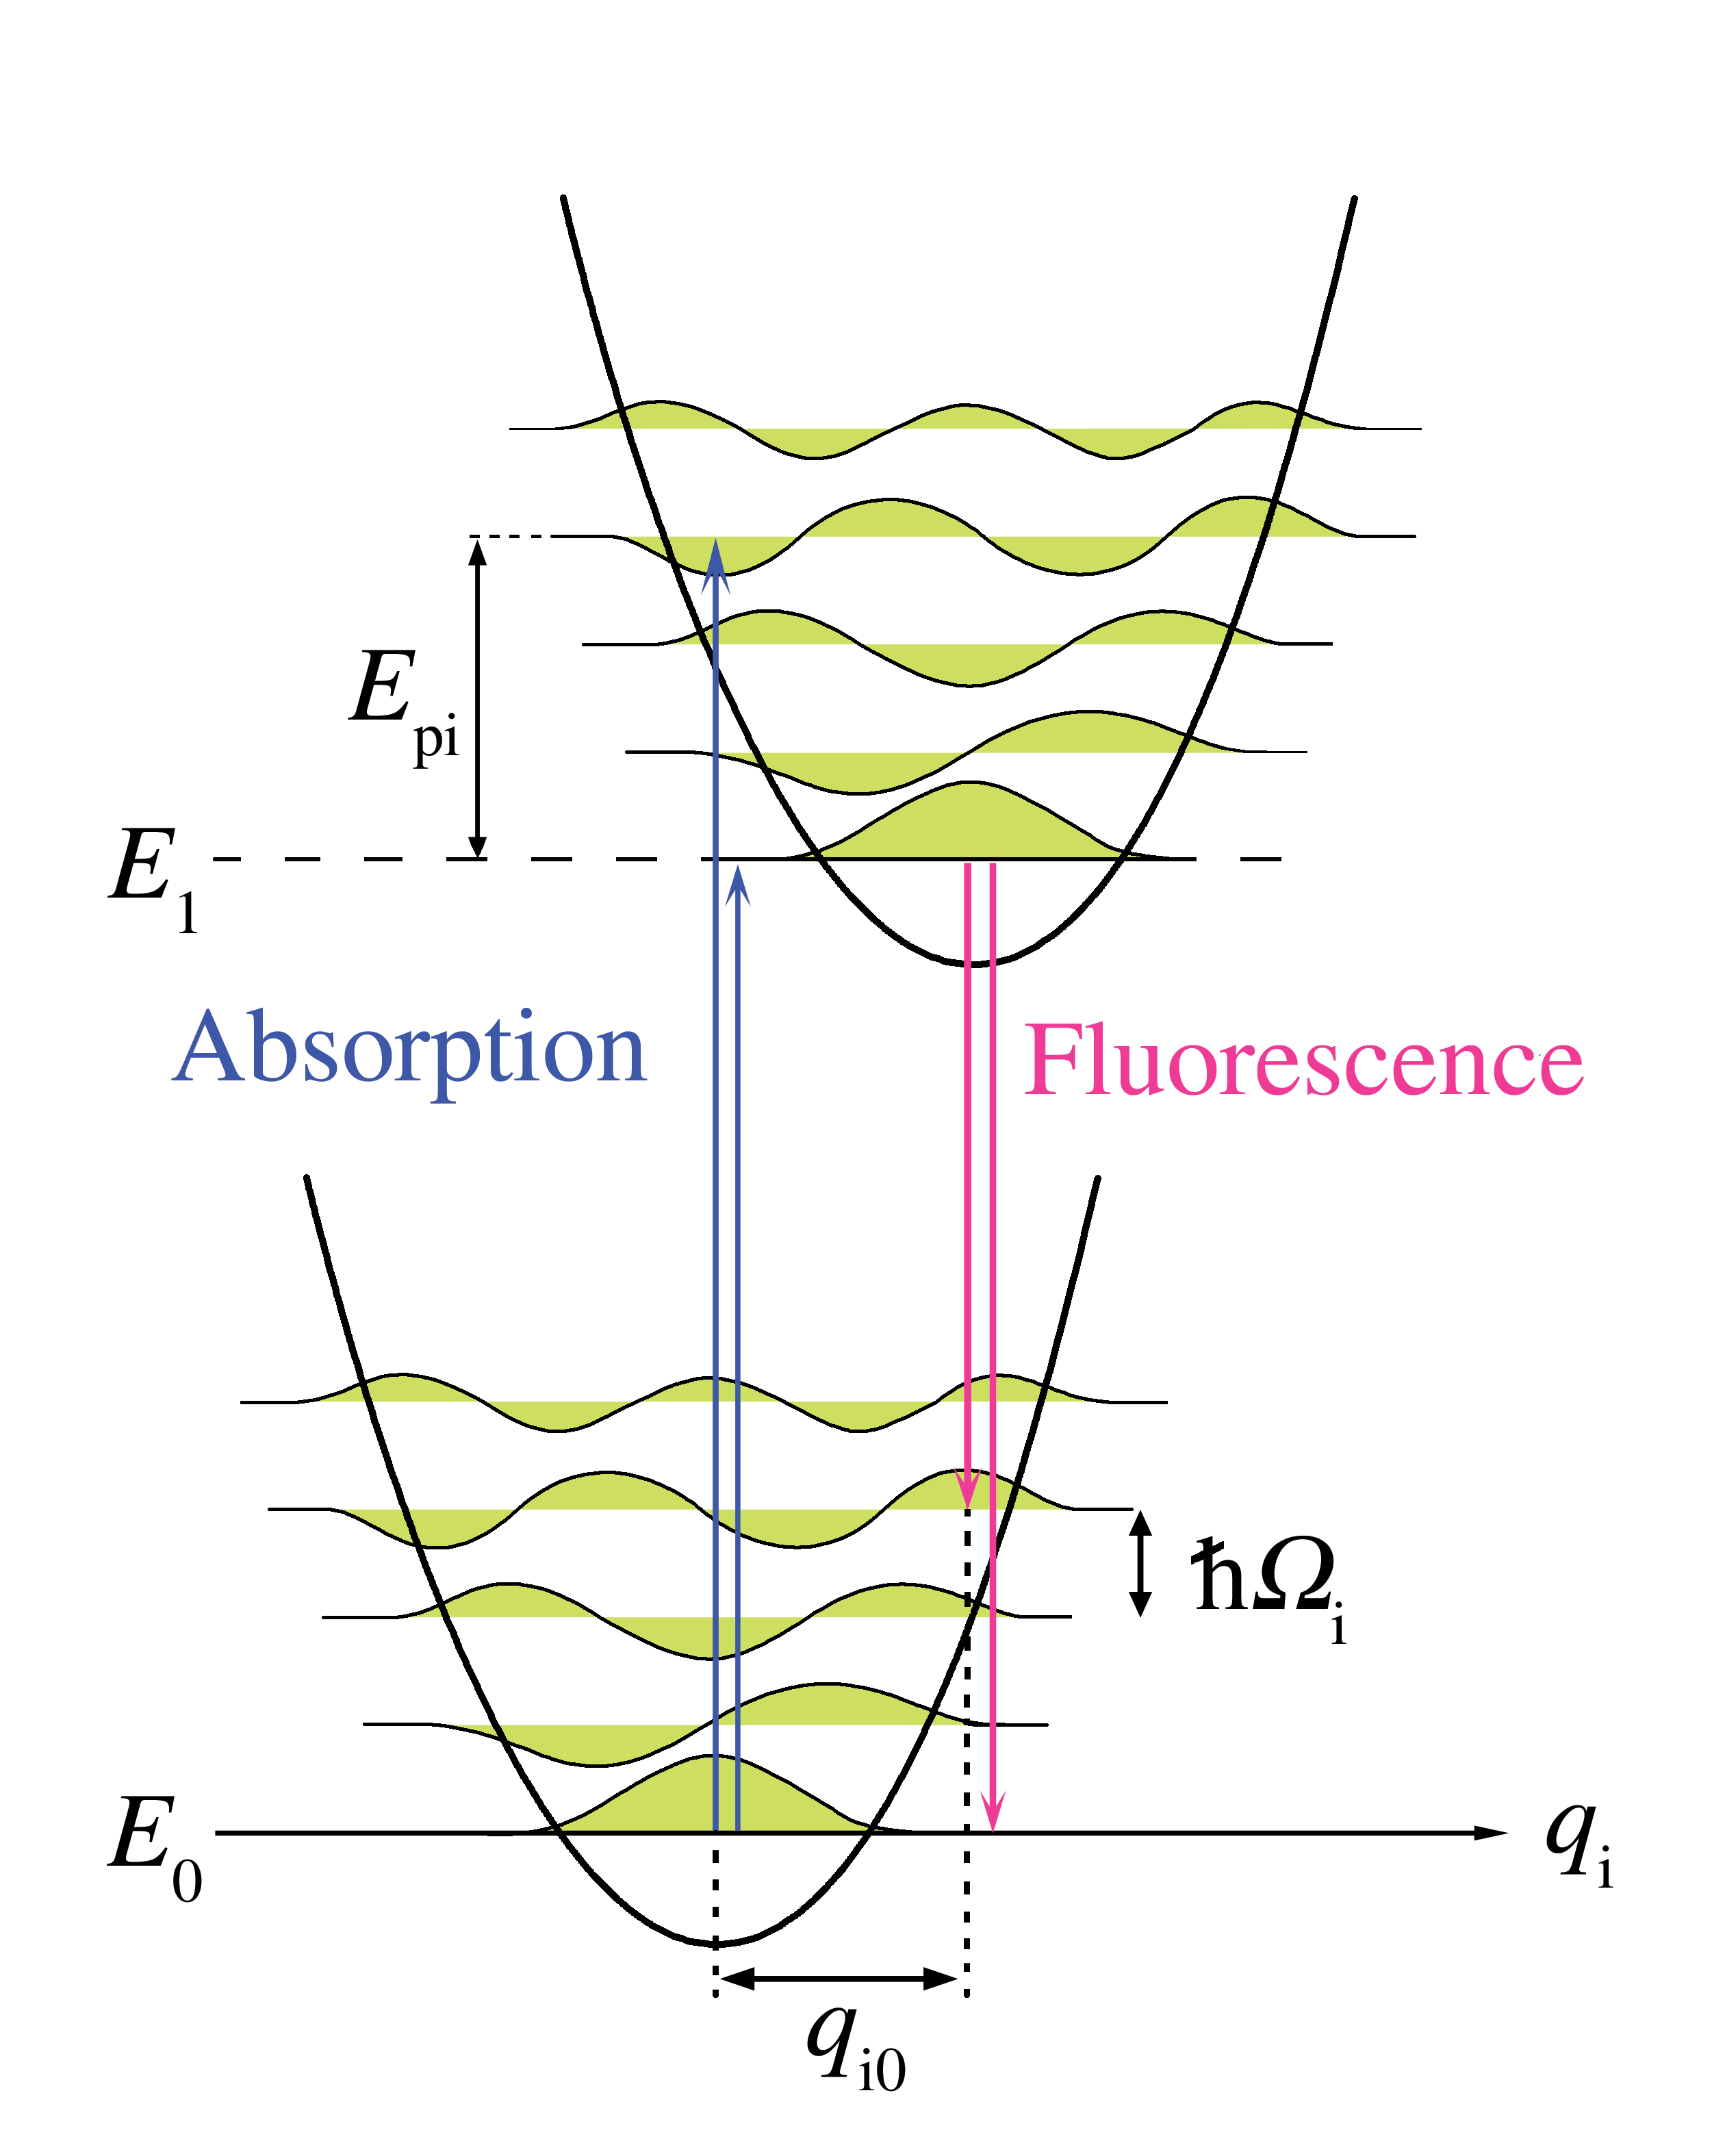
\includegraphics[width=\textwidth]{figures/quantum-dot/Phonon-energy-diagram}
		\caption{Energy spectrum of a two-level electronic system with phonon coupling.
			The arrows describe emission/absorption with and without phonons respectively.~\cite{noauthor_zero-phonon_nodate}}
		\label{fig:phonon-energy-diagram}
	\end{subfigure}%
	~ % An dieser Stelle kann ein zusätzlicher Zwischenraum eingebunden werden: ~, \quad, \qquad, \hfill usw.
	% Eine leere Zeile erzwingt, dass die zweite Grafik darunter erscheint.
	\begin{subfigure}[b]{0.48\textwidth}
		\centering
		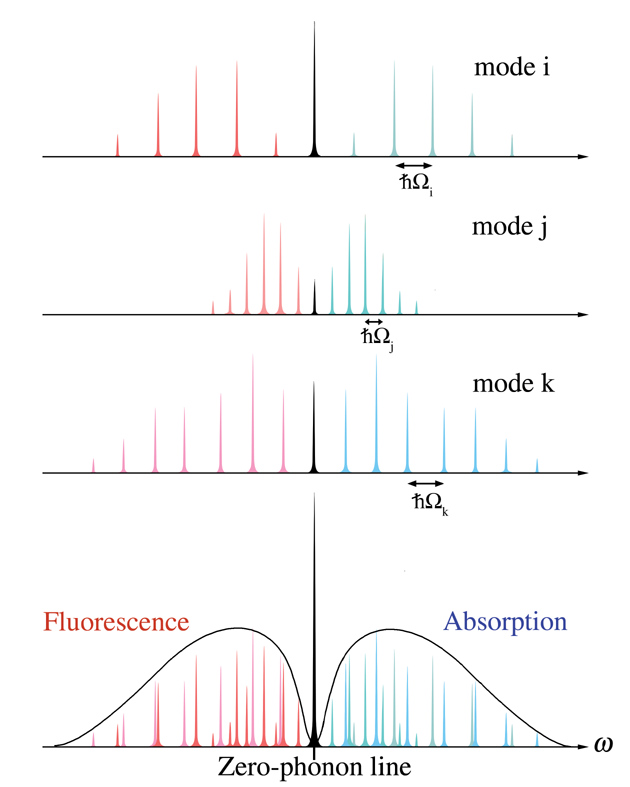
\includegraphics[width=\textwidth]{figures/quantum-dot/Lattice-modes}
		\caption{Three lattice normal modes $(i, j, k)$ and the resulting emission/absorption spectrum.~\cite{noauthor_zero-phonon_nodate}\\}
		\label{fig:lattice-modes}
	\end{subfigure}
	\caption{Zero-phonon line and phonon sideband.}
	\label{fig:zero-phonon-line-phonon-side-band}
\end{figure}
Figure~\ref{fig:phonon-energy-diagram} and \ref{fig:lattice-modes} implicitly assume approximations in addition to the Franck-Condon principles.
The lattice vibrational mode has to be well described by a quantum harmonic oscillator as can be seen in the parabolic shape of the potential wells in figure~\ref{fig:phonon-energy-diagram}.
Additionally, it is assumed that only the lowest lattice vibration is excited and that the harmonic oscillator potentials are equal in both states.

\subsection{Calculate spectral range of zero-phonon line}
A typical lifetime of a GaAs quantum dot is $\Delta t = 250~ps$.
According to the time-energy uncertainty relation
\begin{align}
\Delta E \cdot \Delta t = \frac{h}{2 \pi}\\
\Rightarrow \Delta E = \SI{2.64}{\micro \electronvolt}
\end{align}
The frequency uncertainty can be obtained through
\begin{equation}
\Delta \nu = \frac{\Delta E}{h}
\end{equation}
By developing $\lambda$ into a taylor series
\begin{align}
\label{eq:planck-einstein}
\lambda &= \frac{c}{\nu}\\
\Rightarrow \lambda(\nu) &\approx \lambda(\nu_0) + \lambda'(\nu_0) \cdot (\nu - \nu_0)
\end{align}
$\Delta \lambda$ can be expressed as
\begin{align}
\Delta \lambda &= \lambda(\nu_0 - \Delta \nu) - \lambda(\nu_0)\\
 &= \lambda(\nu_0) - \lambda'(\nu_0)\cdot\Delta \nu - \lambda(\nu_0)\\
 &= - \lambda'(\nu_0)\cdot \Delta \nu.
\end{align}
With equation~\eqref{eq:planck-einstein} this gives
\begin{align}
\Rightarrow \Delta \lambda &= \frac{c}{\nu_0^2} \cdot \Delta \nu = \frac{\lambda_0^2}{c}\cdot\Delta \nu\\
\label{eq:zero-phonon-theoretical-limit}
&\approx \SI{1.0}{\pico \metre}
\end{align}

\subsection{Simulation}

\begin{table}[H]
	\caption[Paramters of GaAs quantum dots used in the laboratory of semiconductor physics department in Linz.]{Parameters of GaAs quantum dots used in the laboratory of semiconductor physics department in Linz.
	Zero-phonon line calculates from from the theoretical limit according to the life time of the excitonic state (as can be seen in equation~\eqref{eq:zero-phonon-theoretical-limit}) up to broader lines which are still valued enough to be measured.
	The phonon sideband resembles data taken from \textcite{scholl_resonance_2019}.}
	\label{tab:quantum-dot-emission}
	\begin{tabular}{@{}llll@{}}
		\toprule
		Quantum dot emission & Center wavelength $\lambda_0$           & Spectral range $\Delta \lambda$ & Waveform                  \\ \midrule
		Zero-phonon line               & \SIrange{700}{800}{\nano \metre} & \SIrange{1.0}{1.4}{\pico \metre} & Cauchy\\
		Phonon sideband       & \SI{\sim 0.25}{\nano \metre} higher than zero-phonon line  & ~\SI{500}{\pico \metre} & Gauss  \\ \bottomrule
	\end{tabular}
\end{table}

The zero-phonon line is described with a Cauchy distribution
\begin{equation}
\Phi_{dot,zero}(\lambda) = \frac{1}{\pi \cdot \Delta\lambda_{zero} \cdot 0.5 \left[1+\left(\frac{\lambda - \lambda_{0, zero}}{\Delta\lambda_{zero} \cdot 0.5}\right)^2\right]}
\end{equation}
with $\lambda_{0, zero}$ as the center wavelength and $\Delta\lambda_{zero}$ as the spectral range of the zero-phonon line.

The phonon side band is described with a Gauss distribution
\begin{equation}
\Phi_{dot,side}(\lambda) = \frac{1}{\sqrt{2\cdot\pi\cdot \Delta\lambda_{side}^2}}\cdot exp\left(-\frac{(\lambda - \lambda_{0, side})^2}{2\cdot \Delta\lambda_{side}^2}\right)
\end{equation}
with $\lambda_{0, side}$ as the center wavelength and $\Delta\lambda_{side}$ as the spectral range of the phonon side band.

\begin{figure}[H]
	\centering
	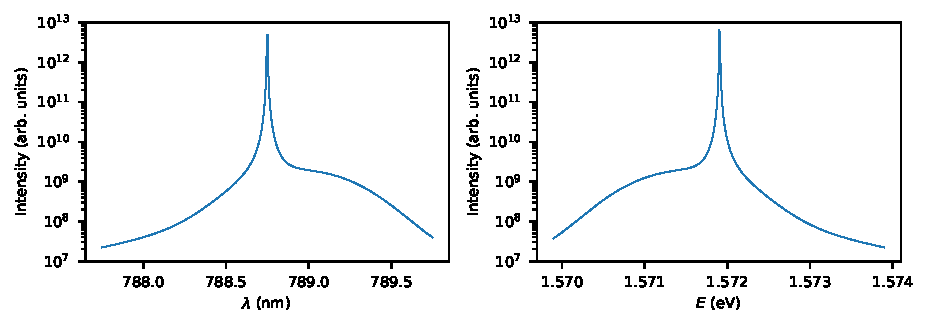
\includegraphics{figures/fabry-perot/plots/quantum_dot_emission_wavelength_energy}
	\caption[Simulated exciton emission of a GaAs quantum dot]{Simulated exciton emission of a GaAs quantum dot plotted dependant on the wavelength $\lambda$ and the Energy $E$.
		The parameters can be found in table~\ref{tab:quantum-dot-emission}.}
	\label{fig:quantumdotemissionwavelengthenergy}
\end{figure}


Dot-Spectra in far field is (TEM$_{00}$).



